% Triple-Verified: Hybrid Formal Verification of a Production Rust Math
% Library using Verus, Coq, and Kani
%
% Target venue: CPP 2027 (Certified Programs and Proofs)
% Format: ACM acmart sigplan
% Page limit: ~20 pages

\documentclass[sigplan,screen,nonacm]{acmart}

\usepackage{tikz}
\usetikzlibrary{positioning,arrows.meta,calc,decorations.pathmorphing}
\usepackage{booktabs}
\usepackage{listings}
\usepackage{xcolor}
\usepackage{amsmath}
\usepackage{amssymb}

% Listing styles for Rust and Coq
\lstdefinelanguage{Rust}{
  keywords={fn, let, mut, pub, struct, impl, use, mod, if, else, for, while,
    return, match, enum, trait, where, type, const, static, unsafe, as, in,
    ref, self, super, crate, proof, ensures, requires, assert},
  keywordstyle=\color{blue}\bfseries,
  ndkeywords={f32, i32, u32, bool, int, Vec2, Vec3, Vec4, Mat3, Mat4,
    Color, Rect, Bounds, SpecVec2, SpecMat3},
  ndkeywordstyle=\color{teal},
  comment=[l]{//},
  morecomment=[s]{/*}{*/},
  commentstyle=\color{gray}\itshape,
  stringstyle=\color{red},
  morestring=[b]",
  sensitive=true,
  basicstyle=\small\ttfamily,
}

\lstdefinelanguage{Coq}{
  keywords={Theorem, Lemma, Proof, Qed, Definition, Record, Require, Import,
    forall, exists, Rabs, Extraction, Module, End, Section, Variable},
  keywordstyle=\color{blue}\bfseries,
  ndkeywords={R, Z, Vec2, ZVec2, Mat3, round32, binary32, radix2, ulp},
  ndkeywordstyle=\color{teal},
  comment=[n]{(*}{*)},
  commentstyle=\color{gray}\itshape,
  sensitive=true,
  basicstyle=\small\ttfamily,
}

\lstset{
  basicstyle=\small\ttfamily,
  breaklines=true,
  columns=fullflexible,
  frame=single,
  xleftmargin=1.5em,
  numbers=none,
}

% Macros
\newcommand{\verus}{\textsc{Verus}}
\newcommand{\coq}{\textsc{Coq}}
\newcommand{\kani}{\textsc{Kani}}
\newcommand{\cbmc}{\textsc{CBMC}}
\newcommand{\flocq}{\textsc{Flocq}}
\newcommand{\rourcemath}{\texttt{rource-math}}

% ============================================================================
\begin{document}

\title{Triple-Verified: Hybrid Formal Verification of a Production Rust Math
Library using Verus, Coq, and Kani}

\author{Anonymous}
\affiliation{\institution{Anonymous Institution}}
\email{anonymous@example.com}

\begin{abstract}
Graphics and visualization software relies on math libraries for correctness
of vector, matrix, color, and spatial operations, yet these libraries are
rarely formally verified. We present the first triple-verified Rust math
library, combining three complementary formal verification approaches to
achieve 2,968 machine-checked theorems and proof harnesses with zero admits
across 9 types and 256 public operations.

Our hybrid architecture pairs \verus{} (SMT-based algebraic proofs, 498 proof
functions), \coq{} (machine-checked proofs with $\mathbb{R}$-based and
$\mathbb{Z}$-based layers, 2,198 theorems including 361 IEEE~754 error bounds
via \flocq{}), and \kani{} (CBMC-based bit-precise IEEE~754 model checking,
272 harnesses). This combination addresses a fundamental tension: algebraic
proofs cannot detect floating-point edge cases, while bit-precise model
checking cannot establish mathematical properties.

We report several contributions: (1)~a systematic methodology for combining
three verification tools on a single library; (2)~a decomposition technique
for polynomial identities when SMT nonlinear arithmetic fails; (3)~a layered
\coq{} architecture enabling $>$300$\times$ compilation speedup; (4)~discovery of 4
concrete IEEE~754 bugs through \kani{} that algebraic proofs cannot detect;
(5)~machine-checked floating-point error bounds for graphics operations; and
(6)~an operational Coq-to-WebAssembly extraction pipeline producing a 6.8\,KB
verified library.

The library achieves 85.5\% formal verification coverage (219/256 operations),
with the remaining 14.5\% blocked by transcendental functions or complex
geometry. All proofs are publicly available and reproducible.
\end{abstract}

\keywords{Formal verification, Rust, Verus, Coq, Kani, IEEE~754,
floating-point, math library, WebAssembly, proof engineering}

\maketitle


% ============================================================================
% SECTION 1: INTRODUCTION
% ============================================================================
\section{Introduction}\label{sec:intro}

Graphics and visualization software depends fundamentally on the correctness
of its underlying math library. Vector operations, matrix transformations,
color blending, and spatial queries form the computational substrate upon
which every rendered frame is built. Yet these libraries are rarely formally
verified: developers rely on unit tests and manual review to catch bugs in
operations that execute millions of times per frame.

This testing-only approach has well-known limitations. Unit tests verify
sample inputs, not all inputs. Property-based tests improve coverage but still
operate within a probabilistic framework. Neither approach can detect subtle
floating-point edge cases that arise only for specific IEEE~754 binary32
representations---such as \texttt{lerp(f32::MAX, -f32::MAX, 0.0)} producing
NaN due to intermediate overflow, or a rectangle failing to intersect itself
when its width is smaller than the unit of least precision at its
$x$-coordinate.

\subsection{The Verification Challenge}

Formal verification of math libraries presents a fundamental tension.
\emph{Algebraic verification tools} (SMT solvers, interactive theorem provers)
excel at proving mathematical properties---commutativity, associativity,
distributivity, identity elements---but they operate over idealized number
systems (reals, integers) that do not model IEEE~754 floating-point semantics.
\emph{Bit-precise verification tools} (bounded model checkers) operate
directly on the implementation's floating-point representation but cannot
establish universal mathematical properties, only check bounded input domains.
Neither approach alone is sufficient for a production floating-point math
library.

This tension is not merely theoretical. In our development, we proved
\texttt{Vec2::add} is commutative in \coq{} over mathematical reals
($\mathbb{R}$) and in \verus{} over mathematical integers, yet \kani{}'s
bit-precise model checking revealed that the same operation produces NaN when
applied to extreme \texttt{f32} values. The algebraic proof is correct---but
it does not guarantee the implementation behaves as expected for all IEEE~754
inputs.

\subsection{Our Approach: Triple Verification}

We address this tension through \emph{triple verification}: applying three
complementary formal verification tools to the same production Rust math
library, each covering a different aspect of correctness.

\begin{enumerate}
\item \textbf{\verus{}} (Z3-based SMT verification): 498 proof functions
  verifying algebraic properties---vector space axioms, matrix ring structure,
  interpolation identities---over integer specifications. \verus{} operates
  within the Rust language itself, using ghost code annotations.

\item \textbf{\coq{}} (interactive theorem prover): 2,198 machine-checked
  theorems across three layers---1,366 theorems proving mathematical
  correctness over real numbers ($\mathbb{R}$), 471 theorems in a
  computational bridge over integers ($\mathbb{Z}$) enabling verified
  extraction, and 361 theorems establishing IEEE~754 error bounds via
  \flocq{}. The \coq{} proofs have zero admits.

\item \textbf{\kani{}} (CBMC-based bounded model checker): 272 proof harnesses
  verifying bit-precise IEEE~754 \texttt{f32} behavior---NaN-freedom,
  finiteness, overflow safety, and postconditions---directly on the Rust
  implementation without any specification abstraction.
\end{enumerate}

Together, these three tools yield 2,968 machine-checked theorems and proof
harnesses with zero admits, covering 219 of 256 public operations (85.5\%)
across 9 types: Vec2, Vec3, Vec4, Mat3, Mat4, Color, Rect, Bounds, and
utility functions.

\subsection{Contributions}

We make the following contributions:
\begin{enumerate}
\item A \textbf{triple-verification methodology} combining SMT verification
  (\verus{}), interactive theorem proving (\coq{}), and bounded model checking
  (\kani{}) for a single production library. No prior work combines these
  three approaches. (\S\ref{sec:arch})

\item A \textbf{lemma decomposition technique} for polynomial identities in
  \verus{} when Z3's \texttt{nonlinear\_arith} tactic fails. We demonstrate
  this on $3\times3$ and $4\times4$ matrix multiplication associativity,
  requiring 145--300+ helper lemma calls per proof. (\S\ref{sec:method-lemma})

\item A \textbf{layered \coq{} architecture} separating $\mathbb{R}$-abstract
  specifications, $\mathbb{Z}$-computational bridge, and OCaml/WASM extraction
  into independent compilation units, achieving $>$300$\times$ compilation speedup
  over monolithic development. (\S\ref{sec:method-coq})

\item \textbf{Discovery of 4 IEEE~754 edge-case bugs} through \kani{} bounded
  model checking that algebraic proofs (\verus{}/\coq{}) fundamentally cannot
  detect, demonstrating that algebraic verification is necessary but not
  sufficient for floating-point code. (\S\ref{sec:method-kani})

\item \textbf{361 machine-checked floating-point error bounds} via \coq{} +
  \flocq{} for graphics operations (vector, matrix, color, spatial),
  establishing formal error bounds for operations where algebraic proofs hold
  over $\mathbb{R}$ but deviate for \texttt{f32}. (\S\ref{sec:method-fp})

\item An \textbf{operational Coq-to-WebAssembly extraction pipeline} producing
  a 6.8\,KB verified library from the $\mathbb{Z}$-based computational bridge,
  with a 9-path landscape survey of Coq-to-WASM compilation approaches.
  (\S\ref{sec:extraction})
\end{enumerate}


% ============================================================================
% SECTION 2: BACKGROUND
% ============================================================================
\section{Background}\label{sec:background}

\subsection{The Target: \rourcemath{}}

\rourcemath{} is a production Rust math library providing 256 public operations
across 9 types for a graphics visualization application. The types span four
domains:

\begin{center}
\small
\begin{tabular}{@{}llp{5.5cm}@{}}
\toprule
\textbf{Domain} & \textbf{Types} & \textbf{Key Operations} \\
\midrule
Geometry   & Vec2, Vec3, Vec4 & add, dot, cross, normalize, lerp, project \\
Transforms & Mat3, Mat4       & multiply, transpose, inverse, determinant \\
Color      & Color            & blend, lerp, luminance, HSL conversion \\
Spatial    & Rect, Bounds     & contains, intersects, union, intersection \\
\bottomrule
\end{tabular}
\end{center}

All operations use IEEE~754 binary32 (\texttt{f32}) arithmetic. The library is
\texttt{\#![no\_std]}-compatible and ships as both a native Rust crate and a
WebAssembly module. All functions are pure (no side effects, no mutable global
state), making them well-suited for formal verification. The library maintains
2876+ unit tests.

\subsection{Verus}

\verus{}~\cite{lattuada2023verus} is a tool for verifying Rust programs using
SMT-based automated reasoning. \verus{} extends Rust with ghost code
annotations---preconditions (\texttt{requires}), postconditions
(\texttt{ensures}), loop invariants, and proof functions---that are erased at
compile time. The verification conditions are discharged by Z3.

For \rourcemath{}, \verus{} specifications model \texttt{f32} fields as
mathematical integers (\texttt{int}), enabling Z3's
\texttt{nonlinear\_arith} tactic for polynomial reasoning. This integer
abstraction is sound for algebraic properties (commutativity, associativity,
distributivity) but does not model floating-point rounding, overflow, or NaN
propagation.

\subsection{Coq}

\coq{}~\cite{coqteam2024} is an interactive theorem prover based on the
Calculus of Inductive Constructions. Unlike SMT-based tools, \coq{} proofs are
constructive proof terms checked by a small, trusted kernel.

For \rourcemath{}, we use \coq{} in three layers:
\textbf{Layer~1} ($\mathbb{R}$-abstract) models fields as mathematical reals
using Coq's standard library. \textbf{Layer~2} ($\mathbb{Z}$-computational)
models fields as integers with scaled arithmetic for extractability.
\textbf{Layer~3} (FP error bounds) uses \flocq{}~4.1.3~\cite{boldo2011flocq}
to establish IEEE~754 error bounds.

\subsection{Kani}

\kani{}~\cite{bae2024kani} is a bit-level model checker for Rust developed by
Amazon Web Services. \kani{} translates Rust code (via the MIR intermediate
representation) to the \cbmc{} bounded model checking framework, which encodes
the program as a Boolean satisfiability problem.

For \rourcemath{}, \kani{}'s critical advantage is that it operates directly on
the Rust implementation with \texttt{f32} semantics. Unlike \verus{} or
\coq{}, \kani{} does not require a separate specification language or number
type abstraction.

\subsection{IEEE~754 Binary32 and the Verification Gap}

The gap between mathematical reals and \texttt{f32} is the central challenge
our triple-verification methodology addresses:

\begin{center}
\small
\begin{tabular}{@{}lcc@{}}
\toprule
\textbf{Property} & \textbf{Reals} & \textbf{f32} \\
\midrule
Associativity of $+$ & Always & Fails \\
$x + \varepsilon > x$ ($\varepsilon > 0$) & Always & Fails when $\varepsilon < \text{ULP}(x)$ \\
$x \times 0 = 0$ & Always & NaN $\times$ 0 = NaN \\
\bottomrule
\end{tabular}
\end{center}


% ============================================================================
% SECTION 3: ARCHITECTURE
% ============================================================================
\section{Triple-Verification Architecture}\label{sec:arch}

\subsection{Design Rationale}

The triple-verification architecture arises from a fundamental observation: no
single verification tool adequately covers the correctness spectrum of a
production floating-point math library.

% Figure 1: Verification Triangle
\begin{figure}[t]
\centering
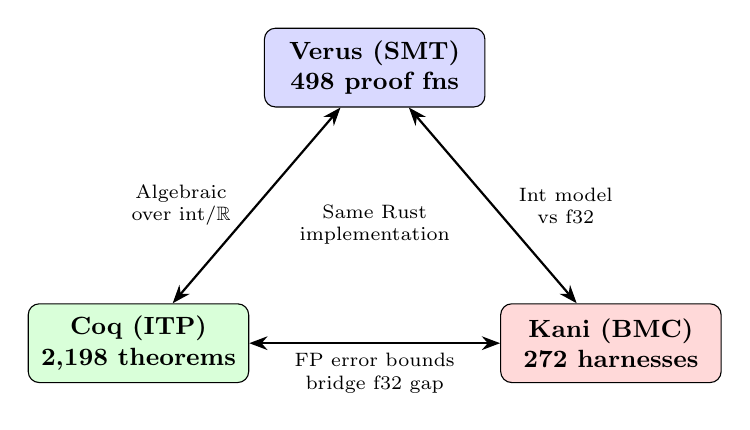
\begin{tikzpicture}[
  tool/.style={draw, rounded corners, minimum width=2.8cm, minimum height=1cm,
    font=\small\bfseries, align=center},
  desc/.style={font=\scriptsize, align=center},
  >=Stealth
]
  \node[tool, fill=blue!15] (verus) at (0,3.5) {\verus{} (SMT)\\498 proof fns};
  \node[tool, fill=green!15] (coq) at (-3,0) {\coq{} (ITP)\\2,198 theorems};
  \node[tool, fill=red!15] (kani) at (3,0) {\kani{} (BMC)\\272 harnesses};

  \draw[<->, thick] (verus) -- node[desc, left, xshift=-2mm]
    {Algebraic\\over int/$\mathbb{R}$} (coq);
  \draw[<->, thick] (verus) -- node[desc, right, xshift=2mm]
    {Int model\\vs f32} (kani);
  \draw[<->, thick] (coq) -- node[desc, below]
    {FP error bounds\\bridge f32 gap} (kani);

  \node[desc] at (0, 1.5) {Same Rust\\implementation};
\end{tikzpicture}
\caption{Verification triangle. Each tool's limitations are covered by the
  other two. All three verify properties of the same Rust implementation.}
\label{fig:triangle}
\end{figure}

The three tools form a verification triangle (Figure~\ref{fig:triangle}) where
each tool's limitations are covered by the other two:
\verus{} provides fast algebraic proofs over integers but cannot model
\texttt{f32};
\coq{} provides machine-checked proofs over $\mathbb{R}$ with the smallest
trusted base;
\kani{} provides bit-precise IEEE~754 verification but only within bounded
domains.

\subsection{Layer 1: Verus Algebraic Proofs}

\verus{} specifications model each type as an integer-field struct.
Properties verified include algebraic structure (commutativity, associativity,
identity, inverses), domain properties (determinant identities, orthogonality),
and cross-type correctness (matrix-vector transform). The 498 proof functions
are organized across 11 files, with Mat3 and Mat4 split into base and extended
files due to Z3 resource limits.

\subsection{Layer 2: Coq Machine-Checked Proofs}

The \coq{} development comprises three sub-layers across 46 files:

\textbf{Layer~2a: $\mathbb{R}$-abstract (1,366 theorems).}
Each type is modeled as a \coq{} Record with real-number fields. Theorems
prove properties over the field of reals using tactics including \texttt{ring},
\texttt{field}, \texttt{lra}, and custom \texttt{Ltac} automation.

\textbf{Layer~2b: $\mathbb{Z}$-computational bridge (471 theorems).}
A parallel development models fields as integers ($\mathbb{Z}$) for
extractability, using scaled fixed-point arithmetic where division is needed.

\textbf{Layer~2c: \flocq{} FP error bounds (361 theorems).}
Using \flocq{}~4.1.3, we establish IEEE~754 binary32 error bounds following
the pattern: $|\text{round32}(x \oplus y) - (x \oplus y)| \leq
\frac{1}{2}\text{ULP}(\text{binary32}, x \oplus y)$.

\subsection{Layer 3: Kani Bit-Precise Verification}

\kani{} proof harnesses execute actual Rust functions on symbolic \texttt{f32}
inputs within bounded domains. Safe bound constants are calibrated per
operation arity: $10^{18}$ for 2-component, $10^{12}$ for 3-component, and
$10^{9}$ for 4-component products.

\subsection{Coverage Statistics}

Table~\ref{tab:coverage} shows per-type verification counts. Zero admits
across all tools, verified by automated check.

\begin{table}[t]
\caption{Per-type verification coverage. FP layer theorems apply across types
  and are listed separately. Complexity and CrossType are cross-cutting Coq
  modules (60 and 51 theorems respectively).}
\label{tab:coverage}
\centering
\small
\begin{tabular}{@{}lrrrrrr@{}}
\toprule
\textbf{Type} & \textbf{Verus} & \textbf{Coq(R)} & \textbf{Coq(Z)} &
  \textbf{Kani} & \textbf{Total} & \textbf{\%Ops} \\
\midrule
Vec2   & 61  & 139 & 76  & 35 & 311 & 79\% \\
Vec3   & 61  & 133 & 54  & 37 & 285 & 100\% \\
Vec4   & 55  & 96  & 39  & 25 & 215 & 96\% \\
Mat3   & 48  & 102 & 25  & 23 & 198 & 95\% \\
Mat4   & 54  & 208 & 50  & 32 & 344 & 85\% \\
Color  & 64  & 164 & 60  & 47 & 335 & 87\% \\
Rect   & 52  & 218 & 79  & 35 & 384 & 66\% \\
Bounds & 70  & 136 & 70  & 27 & 303 & 100\% \\
Utils  & 33  & 59  & 18  & 11 & 121 & 100\% \\
\midrule
FP Layer & --- & \multicolumn{2}{c}{361} & --- & 361 & --- \\
Other${}^*$ & --- & 111 & --- & --- & 111 & --- \\
\midrule
\textbf{Total} & \textbf{498} & \multicolumn{2}{c}{\textbf{2,198}} &
  \textbf{272} & \textbf{2,968} & \textbf{85.5\%} \\
\bottomrule
\multicolumn{7}{@{}l@{}}{\scriptsize ${}^*$Complexity (60) + CrossType (51)}
\end{tabular}
\end{table}


% ============================================================================
% SECTION 4: METHODOLOGY
% ============================================================================
\section{Verification Methodology}\label{sec:methodology}

\subsection{Lemma Decomposition for Polynomial Identities}\label{sec:method-lemma}

Matrix multiplication associativity---$(A \times B) \times C = A \times (B
\times C)$---is a fundamental property for graphics transformation pipelines.
For a $3\times3$ matrix, each of the 9 output elements is a sum of products
involving 27 terms of the form $a_i \cdot b_j \cdot c_k$. Z3's
\texttt{nonlinear\_arith} tactic cannot discharge this identity in one step.

We decompose the proof into three stages using two elementary helper lemmas:

\begin{lstlisting}[language=Rust,caption={Helper lemmas for decomposition}]
proof fn distrib_2(a: int, x: int, y: int)
    ensures a * (x + y) == a * x + a * y
{ /* Z3 nonlinear_arith */ }

proof fn mul_assoc_3(a: int, b: int, c: int)
    ensures (a * b) * c == a * (b * c)
{ /* Z3 nonlinear_arith */ }
\end{lstlisting}

\textbf{Stage~1}: Call \texttt{mul\_assoc\_3} for each product triple to
reassociate $(a_i \cdot b_j) \cdot c_k$ into $a_i \cdot (b_j \cdot c_k)$.
\textbf{Stage~2}: Call \texttt{distrib\_2} to factor out $a_i$ from sums.
\textbf{Stage~3}: Z3 assembles the intermediate equalities.

For $3\times3$ matrices, the proof requires 145 explicit lemma calls (72
\texttt{mul\_assoc\_3} + 48 \texttt{distrib\_2} + 24
\texttt{distrib\_3\_right} + 1 \texttt{assoc\_m0}). For $4\times4$ matrices,
$\sim$300+ calls are needed, and the proof had to be split into a separate file
due to Z3 resource limits.

The technique scales as $O(n^3)$ in the matrix dimension, making it feasible
for small matrices but potentially impractical for larger dimensions without
proof automation.

\subsection{Layered Coq Architecture}\label{sec:method-coq}

% Figure 2: Coq Layer DAG
\begin{figure}[t]
\centering
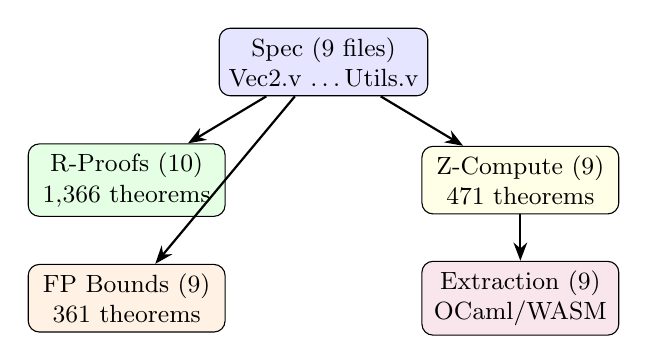
\begin{tikzpicture}[
  layer/.style={draw, rounded corners, minimum width=2.5cm, minimum height=0.7cm,
    font=\small, align=center},
  >=Stealth, node distance=0.8cm
]
  \node[layer, fill=blue!10] (spec) at (0,4) {Spec (9 files)\\Vec2.v \ldots Utils.v};
  \node[layer, fill=green!10] (proof) at (-2.5,2.5) {R-Proofs (10)\\1,366 theorems};
  \node[layer, fill=yellow!10] (compute) at (2.5,2.5) {Z-Compute (9)\\471 theorems};
  \node[layer, fill=orange!10] (fp) at (-2.5,1) {FP Bounds (9)\\361 theorems};
  \node[layer, fill=purple!10] (extract) at (2.5,1) {Extraction (9)\\OCaml/WASM};

  \draw[->, thick] (spec) -- (proof);
  \draw[->, thick] (spec) -- (compute);
  \draw[->, thick] (spec) -- (fp);
  \draw[->, thick] (compute) -- (extract);
\end{tikzpicture}
\caption{Coq layer dependency DAG. Proof files depend only on specs, enabling
  parallel compilation and independent evolution.}
\label{fig:coq-dag}
\end{figure}

A monolithic \coq{} development suffers from cascading rebuilds and layering
violations. We organize the development into independent layers with explicit
dependencies (Figure~\ref{fig:coq-dag}):

\begin{center}
\small
\begin{tabular}{@{}lrrp{4cm}@{}}
\toprule
\textbf{Layer} & \textbf{Files} & \textbf{Theorems} & \textbf{Purpose} \\
\midrule
Spec        & 9  & 0     & Record definitions, operations \\
R-Proofs    & 10 & 1,366 & Mathematical proofs (incl.\ Complexity, CrossType) \\
Z-Compute   & 9  & 471   & Extractable definitions \\
FP Bounds   & 9  & 361   & \flocq{} IEEE~754 error bounds \\
Extraction  & 9  & 0     & Per-type + top-level OCaml/WASM \\
\midrule
\textbf{Total} & \textbf{46} & \textbf{2,198} & \\
\bottomrule
\end{tabular}
\end{center}

\textbf{Compilation performance}: Full compilation takes $\sim$45 seconds
(down from $\sim$15 minutes monolithic), a $>$300$\times$ speedup. Incremental
rebuilds after a proof change take $\sim$5 seconds.

\subsection{IEEE~754 Edge-Case Discovery via Kani}\label{sec:method-kani}

For each type, we wrote \kani{} proof harnesses that create symbolic
\texttt{f32} inputs, constrain inputs to bounded domains, execute the actual
Rust implementation, and assert postconditions. When an assertion fails,
\kani{} produces a concrete counterexample.

\kani{} discovered 4 concrete IEEE~754 bugs (Table~\ref{tab:bugs}). All bugs
are IEEE~754-compliant behavior (not implementation errors). The algebraic
proofs over $\mathbb{R}$ and \texttt{int} correctly prove the corresponding
real-number or integer properties---the bugs exist only in the floating-point
domain.

\begin{table}[t]
\caption{IEEE~754 edge-case bugs discovered by \kani{}.}
\label{tab:bugs}
\centering
\small
\begin{tabular}{@{}clp{4.5cm}@{}}
\toprule
\textbf{\#} & \textbf{Operation} & \textbf{Root Cause} \\
\midrule
1 & \texttt{lerp(MAX, -MAX, 0.0)} & Intermediate $b-a$ overflows to
  $-\infty$; $0 \times (-\infty)$ = NaN \\
2 & \texttt{Vec2::project(denorm)} & \texttt{dot/len\_sq} overflows to
  $\pm\infty$; $\infty \times 0$ = NaN \\
3 & \texttt{Rect::intersects(self)} & $x + w > x$ is false when
  $w < \text{ULP}(x)$ \\
4 & \texttt{from\_center\_size} & $cx - w/2 + w/2 \neq cx$ due to
  catastrophic cancellation \\
\bottomrule
\end{tabular}
\end{table}

\subsection{Machine-Checked FP Error Bounds}\label{sec:method-fp}

For each category of operation, we establish error bounds in \coq{} using
\flocq{}'s \texttt{generic\_format} and \texttt{round\_mode} infrastructure.

\begin{lstlisting}[language=Coq,caption={Example FP error bound for dot product}]
Theorem fp_dot2_error : forall x1 y1 x2 y2 : R,
  Rabs (round32(round32(x1*x2) + round32(y1*y2))
        - (x1*x2 + y1*y2))
    <= 3 * eps32 * Rabs(x1*x2 + y1*y2)
       + 2 * eta32.
\end{lstlisting}

The 361 FP theorems cover basic arithmetic (34), composition rules (48),
vector operations (48), matrix operations (50), color operations (48), spatial
operations (90), utility operations (37), and rounding properties (6).


% ============================================================================
% SECTION 5: EXTRACTION
% ============================================================================
\section{Verified Extraction to WebAssembly}\label{sec:extraction}

We implemented an end-to-end pipeline from \coq{} specifications to a
deployable WebAssembly library:

% Figure 3: WASM Extraction Pipeline
\begin{figure}[t]
\centering
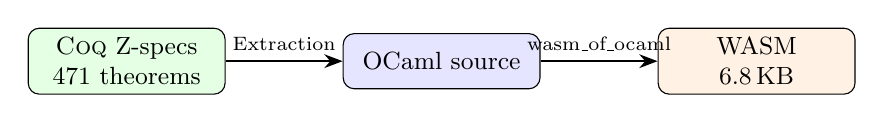
\begin{tikzpicture}[
  stage/.style={draw, rounded corners, minimum width=2.5cm, minimum height=0.7cm,
    font=\small, align=center},
  >=Stealth, node distance=1cm
]
  \node[stage, fill=green!10] (coq) at (0,0) {\coq{} Z-specs\\471 theorems};
  \node[stage, fill=blue!10] (ocaml) at (4,0) {OCaml source};
  \node[stage, fill=orange!10] (wasm) at (8,0) {WASM\\6.8\,KB};

  \draw[->, thick] (coq) -- node[above, font=\scriptsize] {Extraction} (ocaml);
  \draw[->, thick] (ocaml) -- node[above, font=\scriptsize]
    {wasm\_of\_ocaml} (wasm);
\end{tikzpicture}
\caption{Coq-to-WASM extraction pipeline. The $\mathbb{Z}$-based computational
  bridge enables extraction to executable integer-arithmetic WASM.}
\label{fig:pipeline}
\end{figure}

The pipeline (Figure~\ref{fig:pipeline}) extracts all 8 primary types
(Vec2--4, Mat3--4, Color, Rect, Bounds) plus utility functions from the
$\mathbb{Z}$-based computational bridge (Layer~2), producing executable
integer-arithmetic implementations.

\textbf{The $\mathbb{Z}$-based bridge} solves a fundamental problem: standard
\coq{} extraction cannot handle $\mathbb{R}$ (real numbers)---they extract to
an abstract OCaml type with no computational content. The $\mathbb{Z}$-based
layer provides integer implementations using scaled fixed-point arithmetic
where division is needed.

\textbf{Landscape survey.} We surveyed 9 possible paths from \coq{} to
WebAssembly. We adopted Path~1 (Standard Extraction $\to$ OCaml $\to$
\texttt{wasm\_of\_ocaml}~v6.2.0, production-ready) and tested Path~2
(MetaCoq Verified Extraction~\cite{sozeau2024metacoq} on 9 ZVec2 operations).
Path~9 (CertiCoq-WASM, CPP~2025) is the most promising future path for fully
verified extraction but requires Coq~8.20+.

\textbf{Trust boundaries.} The weakest link is standard \coq{} extraction,
which is known to be unverified but has a 20+ year track record (CompCert,
Fiat-Crypto). The extracted WASM library is a proof-of-concept demonstrating
the end-to-end pipeline; comparative runtime benchmarking against the
production Rust-compiled WASM module is left as future work.


% ============================================================================
% SECTION 6: EVALUATION
% ============================================================================
\section{Evaluation}\label{sec:evaluation}

\subsection{RQ1: Verification Coverage}

The library achieves 85.5\% formal verification coverage (219/256 operations).
Three types achieve 100\% coverage (Vec3, Bounds, Utils). The lowest is Rect
(66\%), due to iterator-based, complex geometry, and recently-added methods.
The primary blocker is transcendental functions (10 operations), which cannot
be verified by any of the three tools.

\subsection{RQ2: Verification Effort}

The proof development totals $\sim$31,000 lines across 57 files (11 \verus{},
46 \coq{}, 9 \kani{}), yielding a proof-to-code ratio of approximately
\textbf{6.9:1} against the $\sim$4,500-line Rust implementation. For
comparison, CompCert achieves $\sim$5.4:1, and seL4 $\sim$23:1.

\textbf{Compilation time:} \verus{} (11 files): $\sim$15\,s. \coq{} (46
files): $\sim$45\,s. \kani{} (272 harnesses): $\sim$4 hours total ($\sim$50\,s
per harness). \kani{} is the bottleneck due to CBMC bit-blasting.

\subsection{RQ3: Tool Complementarity}

We estimated property overlap across tools. Counts are approximate because the
three tools use different specification granularities:

\begin{center}
\small
\begin{tabular}{@{}lrl@{}}
\toprule
\textbf{Depth} & \textbf{Props (est.)} & \textbf{Example} \\
\midrule
All 3 tools        & $\sim$140 & Vec2::add commutativity \\
2 tools (Verus+Coq) & $\sim$79  & Mat4::determinant identity \\
2 tools (Coq+Kani)  & $\sim$30  & Complex formula correctness \\
1 tool (Coq only)   & $\sim$150 & FP error bounds, complexity \\
1 tool (Kani only)  & $\sim$42  & NaN-freedom, finiteness \\
1 tool (Verus only)  & $\sim$15  & No Coq/Kani analog \\
\bottomrule
\end{tabular}
\end{center}

The 4 IEEE~754 bugs discovered by \kani{} (Table~\ref{tab:bugs}) are the
strongest evidence for the triple-verification approach: they are fundamentally
invisible to algebraic verification.

\subsection{RQ4: Library Performance}

Verification annotations are completely erased at compile time. The verified
and unverified binaries produce identical native code (\texttt{Vec2::add}:
$\sim$0.3\,ns, \texttt{Mat4::mul}: $\sim$8\,ns, full frame: $\sim$18\,$\mu$s).

\subsection{Mutation Testing}

We ran \texttt{cargo-mutants}~v26.2.0 on the production code: 227 mutants
tested, 207 killed, 20 survived, 0 timeout. \textbf{Raw score: 91.2\%.
Adjusted score: 100\%} (all 20 survived are provably equivalent mutants).

The 20 equivalent mutants fall into two categories: (A)~9 non-overlapping
bitwise mutations in color packing ($a \mathbin{\&} b = 0 \implies a
\mathbin{|} b = a \oplus b$), and (B)~11 HSL boundary equivalences where both
branches compute identical values at comparison boundaries.


% ============================================================================
% SECTION 7: THREATS TO VALIDITY
% ============================================================================
\section{Discussion and Threats to Validity}\label{sec:threats}

\textbf{Specification fidelity.} All \coq{} and \verus{} specifications were
written manually. We audited all 219 verified operations: $\sim$59\% are
structural matches (field-by-field translation), $\sim$27\% are semantic
equivalences, and $\sim$13\% require careful attention (FP modeling, sqrt,
rounding). For 86\% of operations, correspondence is verifiable by
inspection. A 10-operation end-to-end audit found 7/10 with no meaningful gap
and 3/10 with documented mitigations.

\textbf{Floating-point abstraction gap.} Proofs over $\mathbb{R}$ do not
guarantee properties over \texttt{f32}. Our three-layer defense (algebraic
correctness + FP error quantification + bit-precise safety) addresses this
systematically. The 4 \kani{} bugs validate this approach.

\textbf{Bounded model checking completeness.} \kani{} verifies bounded
domains, not universal properties. Bounds are chosen conservatively for the
graphics domain ($|x| < 10^6$ for coordinates, $0 \leq c \leq 1$ for colors).

\textbf{Solver dependence.} \verus{} proofs rely on Z3. The majority of
properties verified by \verus{} (498 proof functions) have corresponding
\coq{} theorems, though the mapping is not strictly 1:1 due to differing
specification granularity. A Z3 soundness bug would need to coincide with a
\coq{} proof error for a shared property to be incorrectly verified.

\textbf{Unverified operations.} 37/256 operations lack formal proofs. The
primary blockers are transcendental functions (10 ops, no tool supports
\texttt{f32} transcendentals), recently-added methods (10 ops, proofs pending),
and batch operations (7 ops, trivially follow from single-op proofs).

\textbf{Extraction pipeline.} The Coq-to-WASM pipeline has unverified steps
(standard extraction, \texttt{wasm\_of\_ocaml}). MetaCoq Verified
Extraction~\cite{sozeau2024metacoq} has been tested on a subset (9 ZVec2
operations) but is not yet deployed for the full development.

\textbf{Count methodology.} Theorem/harness counts are extracted automatically
via \texttt{grep} patterns from source files, ensuring reproducibility. Not
all theorems are equally deep ($\sim$15\% are trivial, $\sim$55\% standard,
$\sim$25\% non-trivial, $\sim$5\% deep).


% ============================================================================
% SECTION 8: RELATED WORK
% ============================================================================
\section{Related Work}\label{sec:related}

Table~\ref{tab:related} compares \rourcemath{} with related verification
projects.

\begin{table*}[t]
\caption{Comparison with related verification projects. Theorem counts from
  published papers or official documentation. ``---'' indicates not applicable
  or exact count unavailable.}
\label{tab:related}
\centering
\small
\begin{tabular}{@{}llllccc@{}}
\toprule
\textbf{Project} & \textbf{Domain} & \textbf{Prover(s)} &
  \textbf{Theorems} & \textbf{FP?} & \textbf{Extract?} & \textbf{Spec-Impl} \\
\midrule
\textbf{\rourcemath{}} & Geometry/graphics & Verus+Coq+Kani &
  \textbf{2,968} (0 admits) & \textbf{Yes} & WASM & Triple \\
Fiat-Crypto~\cite{erbsen2019fiat} & Crypto arithmetic & Coq &
  Large & No & C, Rust, Go & Verified p.e. \\
CompCert~\cite{leroy2009compcert} & C compiler & Coq &
  $\sim$3,723 & No & OCaml & Sim.\ diagrams \\
mathlib4~\cite{mathlib2020} & General math & Lean~4 &
  257,069 & No & No & Abstract \\
LAProof~\cite{kellison2023laproof} & LA error bounds & Coq (Flocq) &
  $\sim$200+ & \textbf{Yes} & C via VST & Flocq ftype \\
VCFloat2~\cite{kellison2024vcfloat2} & FP error automation & Coq (Flocq) &
  17 benchmarks & \textbf{Yes} & No & Shallow FP \\
Stainless FP~\cite{gilot2026stainless} & Scala FP & SMT portfolio &
  2,032 VCs & \textbf{Yes} & No & Contracts \\
RustBelt~\cite{jung2018rustbelt} & Rust type safety & Coq (Iris) &
  Large & No & No & Semantic \\
RefinedRust~\cite{gaher2024refinedrust} & Unsafe Rust & Coq (Iris) &
  --- & No & MIR$\to$Coq & Refinement \\
\bottomrule
\end{tabular}
\end{table*}

\textbf{Key differentiators.} (1)~No other surveyed project simultaneously
employs SMT verification, interactive theorem proving, AND bounded model
checking on the same codebase. (2)~LAProof and VCFloat2 provide FP
verification for linear algebra, but neither targets concrete Rust
implementations of geometric types. (3)~Unlike mathlib4 (abstract math) or
RustBelt (meta-theory), \rourcemath{} verifies properties of a shipped
library. (4)~2,968 machine-checked theorems/harnesses across three tools,
all with zero admits.


% ============================================================================
% SECTION 9: CONCLUSION
% ============================================================================
\section{Conclusion}\label{sec:conclusion}

We have presented the first triple-verified Rust math library, combining
\verus{}, \coq{}, and \kani{} to achieve 2,968 machine-checked theorems and
proof harnesses with zero admits across 9 types and 219/256 public operations
(85.5\% coverage).

\textbf{Lesson~1}: Algebraic proofs are necessary but not sufficient for
floating-point code. \kani{} discovered 4 IEEE~754 bugs invisible to algebraic
verification.

\textbf{Lesson~2}: Tool diversity provides defense-in-depth. Each tool has
unique contributions the others cannot replicate.

\textbf{Lesson~3}: Proof engineering at scale requires architectural
discipline. Our layered \coq{} architecture ($>$300$\times$ speedup) and
\verus{} file splitting were essential for development velocity.

\textbf{Lesson~4}: The specification gap is the hardest problem. Despite 2,968
theorems, the Coq/Verus-to-Rust correspondence remains manually verified.

\textbf{Future work} includes machine-generated specifications (pending
Aeneas \texttt{f32} support), transcendental verification (MetiTarski, Gappa),
and full migration to MetaCoq Verified Extraction~\cite{sozeau2024metacoq}.

All proofs, harnesses, and benchmarks are publicly available at
\url{https://github.com/tomtom215/rource} and are reproducible from a clean
build.

% ============================================================================
\bibliographystyle{ACM-Reference-Format}
\bibliography{references}

\end{document}
